\chapter{Performance}
\label{chap:performance}
I am a chapeter on performance.

%--------------------------------------------------------------------------------------------------------------------------------------------------------------------
%--------------------------------------------------------------------------------------------------------------------------------------------------------------------
%--------------------------------------------------------------------------------------------------------------------------------------------------------------------
%--------------------------------------------------------------------------------------------------------------------------------------------------------------------
%--------------------------------------------------------------------------------------------------------------------------------------------------------------------
%--------------------------------------------------------------------------------------------------------------------------------------------------------------------
%--------------------------------------------------------------------------------------------------------------------------------------------------------------------
\section{Numerical Experiments}
\label{sect:numerical_experiments}

In order to evaluate the interplay between the nonlinear convergence and temporal convergence, two test problems were constructed.
These tests problems were designed to answer the following two questions.

\begin{enumerate}
\item{Does the legacy solver have a converged timestep size insensitive solution similar to that produced by the nonlinear solver for simple problems?}
\item{Do the nonlinear convergence metrics provide a quantifiable measure for the nonlinear convergence of a timestep size insensitive solution?}
\end{enumerate}

\subsection{Geometry}
\label{subsect:experimental_geometry}
For both of the test problems, the same computational geometry was used;  \fig{fig:exp_geometry} represents the experimental geometry.
Each block represents a single continuity cell with a height of 4 [in].
The total height of the channel is 48 [in].
Each continuity cell has a cross-sectional area of 4 [in$^2$].
The red block at the top of the channel represents a boundary cell where the pressure and enthalpy are specified.
It represents an infinite reservoir filled with a fluid at a specified thermodynamic state.
The red triangle represents a specified flow at the bottom edge of the first continuity cell. 

\begin{figure}[h!t]
\begin{center}
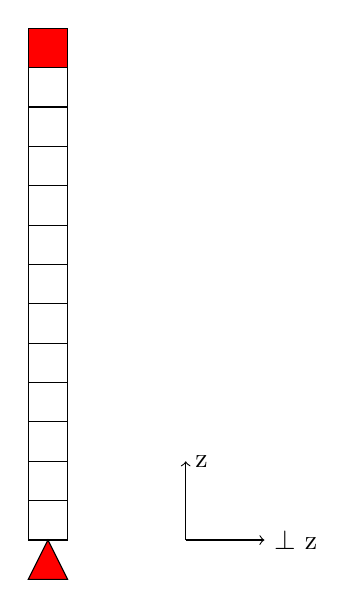
\begin{tikzpicture}
\foreach \x in {1,..., 12} \draw(0, 0.5*\x-0.5) rectangle +(.5,.5);
\filldraw[fill=red] (0, 6) rectangle +(.5,.5); 
\filldraw[fill=red] (0, -0.5) -- (0.25, 0) -- (0.5, -0.5) -- cycle;
\draw[->] (2,0) -- (2, 1) node[anchor=west] {z};
\draw[->] (2,0) -- (3, 0) node[anchor=west] {$\perp$ z};
\end{tikzpicture}
\end{center}
\caption{Geometry for test problems.}
\label{fig:exp_geometry}
\end{figure}

\subsection{Initial and Boundary Conditions}
\label{subsect:ic_bc}

The two problems, while having the same geometry, are different in their dominant physics.
One problem was designed to simulate single-phase, single-field continuous liquid flow in a standpipe.
This problem will be referred to as the single-phase problem.
The second problem was designed such that high-pressure liquid flashes into steam as it enters a standpipe initially filled with saturated vapor at a much lower pressure, known hereafter as the flashing problem.

Table \ref{tab:ic} provides the initial conditions for the two problems.
The pressure, enthalpy, and volume-fractions for the different fields allow for a complete description of the continuity variables.
The initial velocities are set to zero.

\begin{table}[ht]
\centering
\begin{tabular}{@{}lr@{.}lr@{.}lr@{.}lr@{.}lr@{.}l@{}} \toprule
\multirow{2}{*}{Problem} & \multicolumn{2}{c}{Pressure} & \multicolumn{2}{c}{Enthalpy}             & \multicolumn{2}{c}{$\alpha_g$} & \multicolumn{2}{c}{$\alpha_l$} & \multicolumn{2}{c}{$\alpha_e$} \\ 
                         & \multicolumn{2}{c}{[psia]} & \multicolumn{2}{c}{$[\frac{\text{BTU}}{\lbm{}}]$} & \multicolumn{2}{c}{[-]}      & \multicolumn{2}{c}{[-]}      & \multicolumn{2}{c}{[-]}      \\ \midrule
Single-Phase             &  200&0                       &  355&5                                   & 0&0                            & 1&0                            & 0&0 \\
Flashing                 &  200&0                       & 1198&3                                   & 1&0                            & 0&0                            & 0&0 \\ \bottomrule  
\end{tabular}
\caption{Initial conditions for test problems.}
\label{tab:ic}
\end{table}

Each of the problems has a specified pressure-enthalpy boundary condition at the top of the stand pipe and a flow-enthalpy boundary condition at the inlet of the domain.
Table \ref{tab:bc_pe} contains the pressure, enthalpy, and composition of the pressure-enthalpy reservoir. 

\begin{table}[ht]
\centering
\begin{tabular}{@{}lr@{.}lr@{.}lr@{.}lr@{.}lr@{.}l@{}} \toprule
\multirow{2}{*}{Problem} & \multicolumn{2}{c}{Pressure} & \multicolumn{2}{c}{Enthalpy}             & \multicolumn{2}{c}{$\alpha_g$} & \multicolumn{2}{c}{$\alpha_l$} & \multicolumn{2}{c}{$\alpha_e$} \\ 
                         & \multicolumn{2}{c}{[psia]} & \multicolumn{2}{c}{$[\frac{\text{BTU}}{\lbm{}}]$} & \multicolumn{2}{c}{[-]}      & \multicolumn{2}{c}{[-]}      & \multicolumn{2}{c}{[-]}      \\ \midrule
Single-Phase             &  200&0                       &  355&5                                   & 0&0                            & 1&0                            & 0&0 \\
Flashing                 &  200&0                       & 1198&3                                   & 1&0                            & 0&0                            & 0&0 \\ \bottomrule  
\end{tabular}
\caption{The pressure-enthalpy outlet boundary conditions for test problems.}
\label{tab:bc_pe}
\end{table}

The flow-enthalpy boundary condition describes the thermodynamic state of the inflowing fluid and its flow rate.
Table \ref{tab:bc_fe} describes the inlet boundary condition for the two problems.

\begin{table}[ht]
\centering
\begin{tabular}{@{}lr@{.}lr@{.}lr@{.}lr@{.}lr@{.}l@{}} \toprule
\multirow{2}{*}{Problem} & \multicolumn{2}{c}{Pressure} & \multicolumn{2}{c}{Enthalpy}             & \multicolumn{2}{c}{$\alpha_g$} & \multicolumn{2}{c}{$\alpha_l$} & \multicolumn{2}{c}{$\alpha_e$} \\ 
                         & \multicolumn{2}{c}{[psia]} & \multicolumn{2}{c}{$[\frac{\text{BTU}}{\lbm{}}]$} & \multicolumn{2}{c}{[-]}      & \multicolumn{2}{c}{[-]}      & \multicolumn{2}{c}{[-]}      \\ \midrule
Single-Phase             &  200&0                       &  355&5                                   & 0&0                            & 1&0                            & 0&0 \\
Flashing                 & 1000&0                       &  542&6                                   & 1&0                            & 0&0                            & 0&0 \\ \bottomrule  
\end{tabular}
\caption{The flow-enthalpy inlet boundary conditions for test problems.}
\label{tab:bc_fe}
\end{table}

The specified mass flow, $\dot{m}(t)$, at the bottom of the channels is the same for both problems. 
This time-dependent function is given by \eqref{eqn:bc_time_func_single}.

\begin{equation}
\label{eqn:bc_time_func_single}
\dot{m}(t) = \left\{
\begin{array}{cclrcll}
 0.0           & [\frac{ \lbm{} }{\text{s}}] & , &                & t & \leq 1 & [\text{s}] \\
 0.5 ( t - 1)  & [\frac{ \lbm{} }{\text{s}}] & , & 1\; [\text{s}] < & t & \leq 2 & [\text{s}] \\
 0.5           & [\frac{ \lbm{} }{\text{s}}] & , &                & t & > 2    & [\text{s}]
\end{array}\right.
\end{equation}

Both problems adjust their initial pressure distribution to account for hydrostatic head, which is not specified in the input files.
The \cobra{} input files for both problems can be found in \app{app:input_decks}.

\subsection{Procedure}
\label{subsect:procedures}

The two problems were set up so that the maximum allowable timestep was varied.
Each problem was run with the following maximum allowable timesteps: 1 [s], 0.1 [s], 0.01 [s], 0.001 [s], 0.0001 [s], and 0.00001 [s]. 
For the legacy runs, the scaled residuals were evaluated after a single Newton step, $\vec{F}(\vec{x}^{1})$.
For the nonlinear runs, the scaled nonlinear residuals were evaluated at the end of the Newton-loop.
The nonlinear convergence criteria used in the nonlinear solver are described in \sect{sect:nln_solver:cobra}.
The temporal convergence metric was evaluated during post-processing.
In total, there were twenty-four simulations run.
The two different problems were each run at six different maximum timestep sizes on each of the two versions of \cobra{}.

\subsection{Results}
\label{subsect:results}

The results from the simulation runs will now be analyzed to determine the impact of nonlinear convergence upon time-step size sensitivity.
The solutions produced by both solvers will be compared to determine the efficacy of the residual metric in determining the validity of the nonlinear solution.  

Of the twenty-four simulations run, the legacy solver solution of the flashing problem with a \dtmax{} of 1 [s] failed to run to completion.
The timestep limiting procedure outlined in  \sect{sect:algorithmic_concerns} was unable to prevent too large a change in the independent parameters by reducing the timestep.
This caused the problem to try to run below the minimum allowable timestep size, which resulted in the software aborting.
However, the nonlinearly convergent \cobra{} was able to run at a \dtmax{} of 1 [s].
Both versions of \cobra{} are subject to the same limits on change of independent variables.

For the flashing problem, the parameter of interest for temporal convergence testing is $\alpha_g$ at 2 [in] from the inlet of the stand pipe.
\fig{fig:flashing_1em1} shows the gaseous volume fraction 2 [in] from the inlet of the stand pipe as a function of time for a \dtmax{} of 1.0E-1 [s] for both the legacy and the nonlinear solvers.

%\begin{figure}[h!t]
%\centering
%\subfloat[Solution with \dtmax{} = 1.0E-1 {[s]}]{\includegraphics[width=0.49\textwidth]{images/flashing_1em1.eps}
%\label{fig:flashing_1em1}}
%\subfloat[Solution with \dtmax{} = 1.0E-5 {[s]}]{\includegraphics[width=0.49\textwidth]{images/flashing_1em5.eps}
%\label{fig:flashing_1em5}}
%\caption[Flashing solution at \dtmax{} = 1.0E-1 {[s]}and 1.0E-5 {[s]}]{Flashing solution at \dtmax{} = 1.0E-1 {[s]} and 1.0E-5 {[s]}.}
%\label{fig:flashing_compare_1}
%\end{figure}

\begin{figure}[h!t]
\centering
\includegraphics[width=0.94\textwidth]{images/flashing_1em1.eps}
\caption{Flashing solution at \dtmax{} = 1.0E-1 {[s]}}
\label{fig:flashing_1em1}
\end{figure}

\begin{figure}[h!t]
\centering
\includegraphics[width=.94\textwidth]{images/flashing_1em5.eps}
\caption{Flashing solution at \dtmax{} = 1.0E-5 {[s]}.}
\label{fig:flashing_1em5}
\end{figure}

Note that the nonlinearly resolved solution is qualitatively different than the legacy single-shot solution, \fig{fig:flashing_1em1}.
Even as the \dtmax{} is reduced, this discrepancy does not disappear, \fig{fig:flashing_1em5}.
The two solutions do not converge to the same solution as the timestep size was reduced.
However, the solution to the flashing problem produced by the nonlinear solver, \fig{fig:nl_mode_flashing}, qualitatively varies less as the timestep size is reduced than that produced by the legacy solver, \fig{fig:cobra_mode_flashing}.
However, both \fig{fig:cobra_mode_flashing} and \fig{fig:nl_mode_flashing} show that as the timestep size is reduced the two different solutions become more timestep size insensitive.

%\begin{figure}[h!t]
%\centering
%\subfloat[Legacy mode solution.]{\includegraphics[width=0.49\textwidth]{images/cobra_flashing_al_2in.eps}
%\label{fig:cobra_mode_flashing}}
%\subfloat[Nonlinear mode solution.]{\includegraphics[width=0.49\textwidth]{images/nl_flashing_al_2in.eps}
%\label{fig:nl_mode_flashing}}
%\caption{Flashing simulation.}
%\label{fig:flashing_solutions_1}
%\end{figure}

\begin{figure}[h!t]
\centering
\includegraphics[width=.94\textwidth]{images/cobra_flashing_al_2in.eps}
\caption{Legacy solver flashing solution.}
\label{fig:cobra_mode_flashing}
\end{figure}

\begin{figure}[h!t]
\centering
\includegraphics[width=.94\textwidth]{images/nl_flashing_al_2in.eps}
\caption{Nonlinear solver flashing solution.}
\label{fig:nl_mode_flashing}
\end{figure}

The two solvers, when applied to the same problem that contains highly nonlinear physics, produce two different timestep size invariant solutions.
These two solutions achieve qualitative timestep size invariance at different timestep sizes.
The parameter of interest in the solution produced by the nonlinear solver with a 1 [s] $\Delta t_{\text{MAX}}$ is qualitatively close to that produced with a 0.1 [s] $\Delta t_{\text{MAX}}$, \fig{fig:nl_flashing_compare}.
The same level of qualitative timestep size invariance is achieved in the legacy solver solutions between a \dtmax{} of 1.0E-3 [s] and 1.0E-4 [s], \fig{fig:cobra_flashing_compare}.

%\begin{figure}[h!t]
%\centering
%\subfloat[Nonlinear mode solution.]{\includegraphics[width=0.49\textwidth]{images/nl_flashing_1em0_1em1.eps}
%\label{fig:nl_flashing_compare}}
%\subfloat[Legacy mode solution.]{\includegraphics[width=0.49\textwidth]{images/cobra_flashing_1em1_1em4.eps}
%\label{fig:cobra_flashing_compare}}
%\caption{Timestep size insensitive flashing solutions.}
%\label{fig:flashing_res_comp_1}
%\end{figure}

\begin{figure}[h!t]
\centering
\includegraphics[width=.94\textwidth]{images/nl_flashing_1em0_1em1.eps}
\caption{Nonlinear solver timestep size insensitive flashing solution.}
\label{fig:nl_flashing_compare}
\end{figure}

\begin{figure}[h!t]
\centering
\includegraphics[width=.94\textwidth]{images/cobra_flashing_1em1_1em4.eps}
\caption{Legacy solver timestep size insensitive flashing solution.}
\label{fig:cobra_flashing_compare}
\end{figure}

The timestep size insensitive solution produced by the nonlinear solver occurs at a maximum timestep size three orders of magnitude greater than that achieved by the legacy solver in \cobra{}.
An examination of the nonlinear residual over the course of the transient provides insight into why this behavior is observed.
The scaled residual for the legacy flashing problem indicates that, even for small timestep sizes, the solution obtained still does not satisfy the discrete nonlinear equations, \fig{fig:legacy_flashing_residual}.
This is in contrast to the nonlinear flashing problem, which shows a lower residual over the course of the simulation, \fig{fig:nonlinear_flashing_residual}.

%\begin{figure}[h!t]
%\centering
%\subfloat[Legacy solver residuals.]{\includegraphics[width=0.49\textwidth]{images/cobra_flashing_res_compare.eps}
%\label{fig:legacy_flashing_residual}}
%\subfloat[Nonlinear solver residuals.]{\includegraphics[width=0.49\textwidth]{images/nl_flashing_res_compare.eps}
%\label{fig:nonlinear_flashing_residual}}
%\caption[Flashing residual at $\Delta t_{\text{MAX}}$ = 1.0E-1 {[s]}and 1.0E-5 {[s]}]{Flashing residual at $\Delta t_{\text{MAX}}$ = 1.0E-1 {[s]} and 1.0E-5 {[s]}.}
%\label{fig:flashing_compare_2}
%\end{figure}

\begin{figure}[h!t]
\centering
\includegraphics[width=0.94\textwidth]{images/cobra_flashing_res_compare.eps}
\caption{Residual of the flashing solution for the legacy solver.}
\label{fig:legacy_flashing_residual}
\end{figure}

\begin{figure}[h!t]
\centering
\includegraphics[width=0.94\textwidth]{images/nl_flashing_res_compare.eps}
\caption{Residual of the flashing solution for the nonlinear solver.}
\label{fig:nonlinear_flashing_residual}
\end{figure}

The reduction in the residual exhibited by the solution produced by the legacy solver, \fig{fig:legacy_flashing_residual}, shows that the reduction of the maximum allowable timestep size now serves two purposes.
The first is that as \dtmax{} is reduced the nonlinear physics are being better resolved; however, even for small maximum allowable timestep sizes, the residuals are still large compared to those of the nonlinear solution, \fig{fig:nonlinear_flashing_residual}.
The second purpose in reducing \dtmax{} is to decrease the error due to the discrete approximation of the temporal integral of the governing equations.
While the reduction of the maximum timestep size in the legacy solver serves the purpose of reducing the residual, the nonlinear solver performs this task naturally.
Therefore, in the nonlinear solver the reduction of the maximum timestep size primarily serves to reduce the error from the approximate discrete temporal integral.

During simulations with large \dtmax{} there are three time periods of the transient where the residuals from the nonlinear solver are nontrivial.
These are at the initiation of the inlet flow, during the 1 [s] long ramp to full flow, and after the inlet flow has achieved steady state at 2 [s].
The convergence criteria outlined in \sect{sect:nln_solver:cobra} include two paths through which Newton's method may terminate while having a non-trivial residual.
The first is that the maximum allowable number of Newton iterates, $k_{\text{MAX}}$, may have been exceeded. 
This may indicate that $k_{\text{MAX}}$ may be too small, terminating the iterative process prior to a solution being obtained.
The second is that the norm of the scaled independent parameter update vector may be below its convergence threshold.
A concern is that the update vector produced by the Newton step may be truncated based upon the limiting of the independent parameters at the end of a Newton step.
It may be impossible for the algorithm to reach a nonlinearly converged solution without pushing an independent parameter outside of the acceptable limits imposed by the software.
Since the global minimization problem is not formulated as a constrained minimization problem, there may be inconsistencies in the solution.
This non-convergence of the residual needs additional investigation to determine its cause, its impact upon the algorithmic framework, and its possible remedies.

%\begin{figure}[h!t]
%\centering
%\subfloat[\dtmax{} = 1.0 {[s]}]{\includegraphics[width=0.49\textwidth]{images/single_1em0.eps}
%\label{fig:single_1em1}}
%\subfloat[\dtmax{} = 1.0E-5 {[s]}]{\includegraphics[width=0.49\textwidth]{images/single_1em5.eps}
%\label{fig:single_1em5}}
%\caption[Single-phase solution at \dtmax{} = 1.0 {[s]}and 1.0E-5 {[s]}]{Single-phase solution with \dtmax{} = 1.0 {[s]} and 1.0E-5 {[s]}.}
%\label{fig:single_compare_1}
%\end{figure}

\begin{figure}[h!t]
\centering
\includegraphics[width=0.94\textwidth]{images/single_1em0.eps}
\caption{Single-phase solution with \dtmax{} = 1.0 {[s]}.}
\label{fig:single_1em1}
\end{figure}

\begin{figure}[h!t]
\centering
\includegraphics[width=0.94\textwidth]{images/single_1em5.eps}
\caption{Single-phase solution with \dtmax{} = 1.0E-5 {[s]}.}
\label{fig:single_1em5}
\end{figure}

The single-phase case was designed to test if the legacy solver produced a simulation result that was equivalent to that produced by the nonlinear solver.
More specifically, it was designed to show that for problems where the physics of interest have relatively low nonlinearities, the legacy solver provides as accurate a solution as the nonlinear solver.
\fig{fig:single_1em1} and \fig{fig:single_1em5} show the solution produced by both the nonlinear and legacy solvers of \cobra{}.
Unlike the flashing problem, both solvers were able to solve the problem for all of the \dtmax{} specified.
The solutions produced by both solvers are qualitatively equivalent at \dtmax{} = 1.0 [s] and \dtmax{} = 1.0E-5 [s].
This indicates that the legacy solver is adequate in regions where the solution is not highly nonlinear.

%\begin{figure}[h!t]
%\centering
%\subfloat[Legacy mode.]
%{\includegraphics[width=0.49\textwidth]{images/cobra_single_res_v_dt.eps}
%\label{fig:leg_single_res}}
%\subfloat[Nonlinear mode.]{\includegraphics[width=0.49\textwidth]{images/nl_single_res_v_dt.eps}
%\label{fig:nl_single_res}}
%\caption[Single-phase residuals.]{Single-phase residuals.}
%\label{fig:single_compare_2}
%\end{figure}

\begin{figure}[h!t]
\centering
\includegraphics[width=0.94\textwidth]{images/cobra_single_res_v_dt.eps}
\caption{Legacy solver single-phase residuals.}
\label{fig:leg_single_res}
\end{figure}

\begin{figure}[h!t]
\centering
\includegraphics[width=0.94\textwidth]{images/nl_single_res_v_dt.eps}
\caption{Nonlinear solver single-phase residuals.}
\label{fig:nl_single_res}
\end{figure}

Examining the residual for the two different solvers will provide insight into how well each of them are at solving the nonlinear problem.
The residual of the legacy solver solution for the single-phase problem, \fig{fig:leg_single_res}, shows that the nonlinear residuals are nontrivial during two periods of the transient.
The first region of nontrivial residuals is present only for larger values of \dtmax{} and occurs when the the inlet flow initiates at 1 [s].
The second region occurs at smaller values of \dtmax{} and occurs near the beginning of the transient.
For the nonlinear solver solution residuals, \fig{fig:nl_single_res}, the same two regions, the start of simulation and the inlet flow initialization, exhibit similar nontrivial residuals.
However, the behavior of the residual for the nonlinear solver as a function of \dtmax{} exhibits an anomaly that is absent in the legacy solver.
To put the anomaly in context it should first be noted that the nonlinear residual at the initiation of the ramp is approximately zero for \dtmax{} = 1 [s] and \dtmax{} = 1.0E-5 [s].
It is only during intermediate values of \dtmax{} that the residuals becomes nontrivial during the ramp initiation.

%\begin{figure}[h!t]
%\centering
%\subfloat[Transient Solution]{\includegraphics[width=0.49\textwidth]{images/single_1em3.eps}
%\label{fig:single_1em3}}
%\subfloat[Zoomed Solution]{\includegraphics[width=0.49\textwidth]{images/single_1em3_zoom.eps}
%\label{fig:single_1em3_zoom}}
%\caption[Single-phase solution at \dtmax{} = 1.0E-3 {[s]}]{Single-phase solution with \dtmax{} = 1.0E-3 {[s]}.}
%\label{fig:single_compare_3}
%\end{figure}

\begin{figure}[h!t]
\centering
\includegraphics[width=0.94\textwidth]{images/single_1em3.eps}
\caption{Full transient single-phase solution with \dtmax{} = 1.0E-3 {[s]}.}
\label{fig:single_1em3}
\end{figure}

\begin{figure}[h!t]
\centering
\includegraphics[width=0.94\textwidth]{images/single_1em3_zoom.eps}
\caption{Zoomed single-phase solution with \dtmax{} = 1.0E-3 {[s]}.}
\label{fig:single_1em3_zoom}
\end{figure}

While the solutions at \dtmax{} = 1.0 [s] and \dtmax{} = 1.0E-5 [s] are identical for the two solver modes, the solutions at intermediate timestep sizes were not identical.
In particular, the nonlinear solver produces a solution at \dtmax{} = 1.0E-3 [s] that is inconsistent with both the solution produced by the legacy solver and, more importantly, with the specified inlet boundary conditions.
The two solvers produce solutions that agree for most of the domain, \fig{fig:single_1em3}, except at the initiation of the inlet flow at 1 [s], \fig{fig:single_1em3_zoom}.

%\begin{figure}[h!t]
%\centering
%\includegraphics[width=0.49\textwidth]{images/nl_res_single_zoom.eps}
%\caption{Nonlinear mode solution residual for single-phase problem.}
%\label{fig:nl_res_single_zoom}
%\end{figure}

\begin{figure}[h!t]
\centering
\includegraphics[width=0.94\textwidth]{images/nl_res_single_zoom.eps}
\caption{Zoomed residuals for the single-phase solution from the nonlinear solver.}
\label{fig:nl_res_single_zoom}
\end{figure}

This difference is manifested in the residuals for the nonlinear solver solution around 1 [s], \fig{fig:nl_res_single_zoom}.
The residual at the time of inlet flow initialization has a marked increase between the \dtmax{} = 1.0E-3 and \dtmax{} = 1.0E-2 solutions.
The reason for this behavior is, as of yet, unknown.
It is likely related to the same nonlinear non-convergence behavior remarked upon for the flashing problem. 

One way to quantify the difference between the solutions is by measuring the residual convergence metrics outlined in \sect{sect:temporal_convergence}.
These metrics provide a measure of how poorly the discrete nonlinear equations are being solved at every timestep in the transient.
The resolution of the residual allows for a solution that is less sensitive to timestep size selection than for a solution that does not resolve the residual.
The convergence metrics will be used to determine if a qualitative temporal-convergence determination can lead to the acceptance of a solution that is not nonlinearly converged.

For each of the test cases, the two different metrics were compared at the different \dtmax{}.
To examine efficacy of the the temporal convergence criteria, both the average and moment based temporal convergence criteria were evaluated for each of the twenty-three successful simulations.
The values of these metrics will be compared between different solvers for the same test problem. 

The two different nonlinear convergence metrics will now be examined for the flashing problem.
\tab{tab:flashing_criteria} shows both the average metric, $\tilde{R}$, and the moment based metric, $\tilde{R}_{\text{M}}$.
The entry for the legacy mode solution at 1 [s] is empty, reflecting its inability to solve the problem.
For the nonlinear solver, both metrics are decreasing as the \dtmax{} is decreased.
While the legacy solver also shows a decreasing residual metric, it does not decrease in order-of-magnitude, indicating that as the \dtmax{} is reduced the nonlinearities in the problem are not being sufficiently resolved.

\begin{table}[h!t]
\centering
\begin{tabular}{@{}l r@{.}l r@{.}l r@{.}l r@{.}l @{}}
\toprule
& \multicolumn{4}{c}{$\tilde{R}$} & \multicolumn{4}{c}{$\tilde{R}_{\text{M}}$}  \\
$\dtmax{}$ & \multicolumn{2}{c}{Legacy} & \multicolumn{2}{c}{Nonlinear} & \multicolumn{2}{c}{Legacy}& \multicolumn{2}{c}{Nonlinear}  \\
\midrule
1.0    & \multicolumn{2}{c}{-} & 1&177E-3 & \multicolumn{2}{c}{-} & 6&885E-4 \\
1.0E-1 & 5&487E-2 & 1&141E-3 & 5&044E-2 & 6&730E-4 \\
1.0E-2 & 4&960E-2 & 3&413E-4 & 4&570E-2 & 2&511E-4 \\
1.0E-3 & 3&172E-2 & 2&669E-4 & 2&372E-2 & 1&975E-4 \\
1.0E-4 & 2&504E-2 & 1&346E-4 & 1&838E-2 & 8&974E-5 \\
1.0E-5 & 2&166E-2 & 5&075E-5 & 1&922E-2 & 4&581E-5 \\
\bottomrule  
\end{tabular}
\caption{Nonlinear convergence metrics for flashing problem.}
\label{tab:flashing_criteria}
\end{table}

\begin{table}[h!t]
\centering
\begin{tabular}{@{}l r@{.}l r@{.}l r@{.}l r@{.}l @{}}
\toprule
& \multicolumn{4}{c}{$\tilde{R}$} & \multicolumn{4}{c}{$\tilde{R}_{\text{M}}$}  \\
$\dtmax{}$ & \multicolumn{2}{c}{Legacy} & \multicolumn{2}{c}{Nonlinear} & \multicolumn{2}{c}{Legacy}& \multicolumn{2}{c}{Nonlinear}  \\
\midrule
1.0    & 3&149E-3 & 1&700E-3 & 1&485E-3 & 1&070E-4 \\
1.0E-1 & 2&866E-3 & 1&700E-3 & 1&287E-3 & 1&070E-4 \\
1.0E-2 & 3&412E-4 & 1&357E-3 & 1&417E-4 & 7&701E-5 \\
1.0E-3 & 2&207E-4 & 4&584E-4 & 8&805E-5 & 1&178E-4 \\
1.0E-4 & 1&672E-4 & 1&588E-3 & 1&834E-5 & 4&958E-5 \\
1.0E-5 & 5&493E-4 & 2&758E-4 & 1&916E-5 & 8&939E-5 \\
\bottomrule  
\end{tabular}
\caption{Nonlinear convergence metrics for the single-phase problem.}
\label{tab:single_criteria}
\end{table}

\tab{tab:single_criteria} shows the two metrics for the single-phase problem.
Since the single-phase problem is relatively linear, the legacy solver produces metrics that are on the same order as those for the nonlinear solver.
Due to the non-convergence of the nonlinear solver at \dtmax{} = 1.0E-3, the moment based metric for the nonlinear solver is greater than the equivalent legacy solver metric.
